\renewcommand{\captiontitle}{变换误差}
\begin{sidewaysfigure*}
\begin{center}
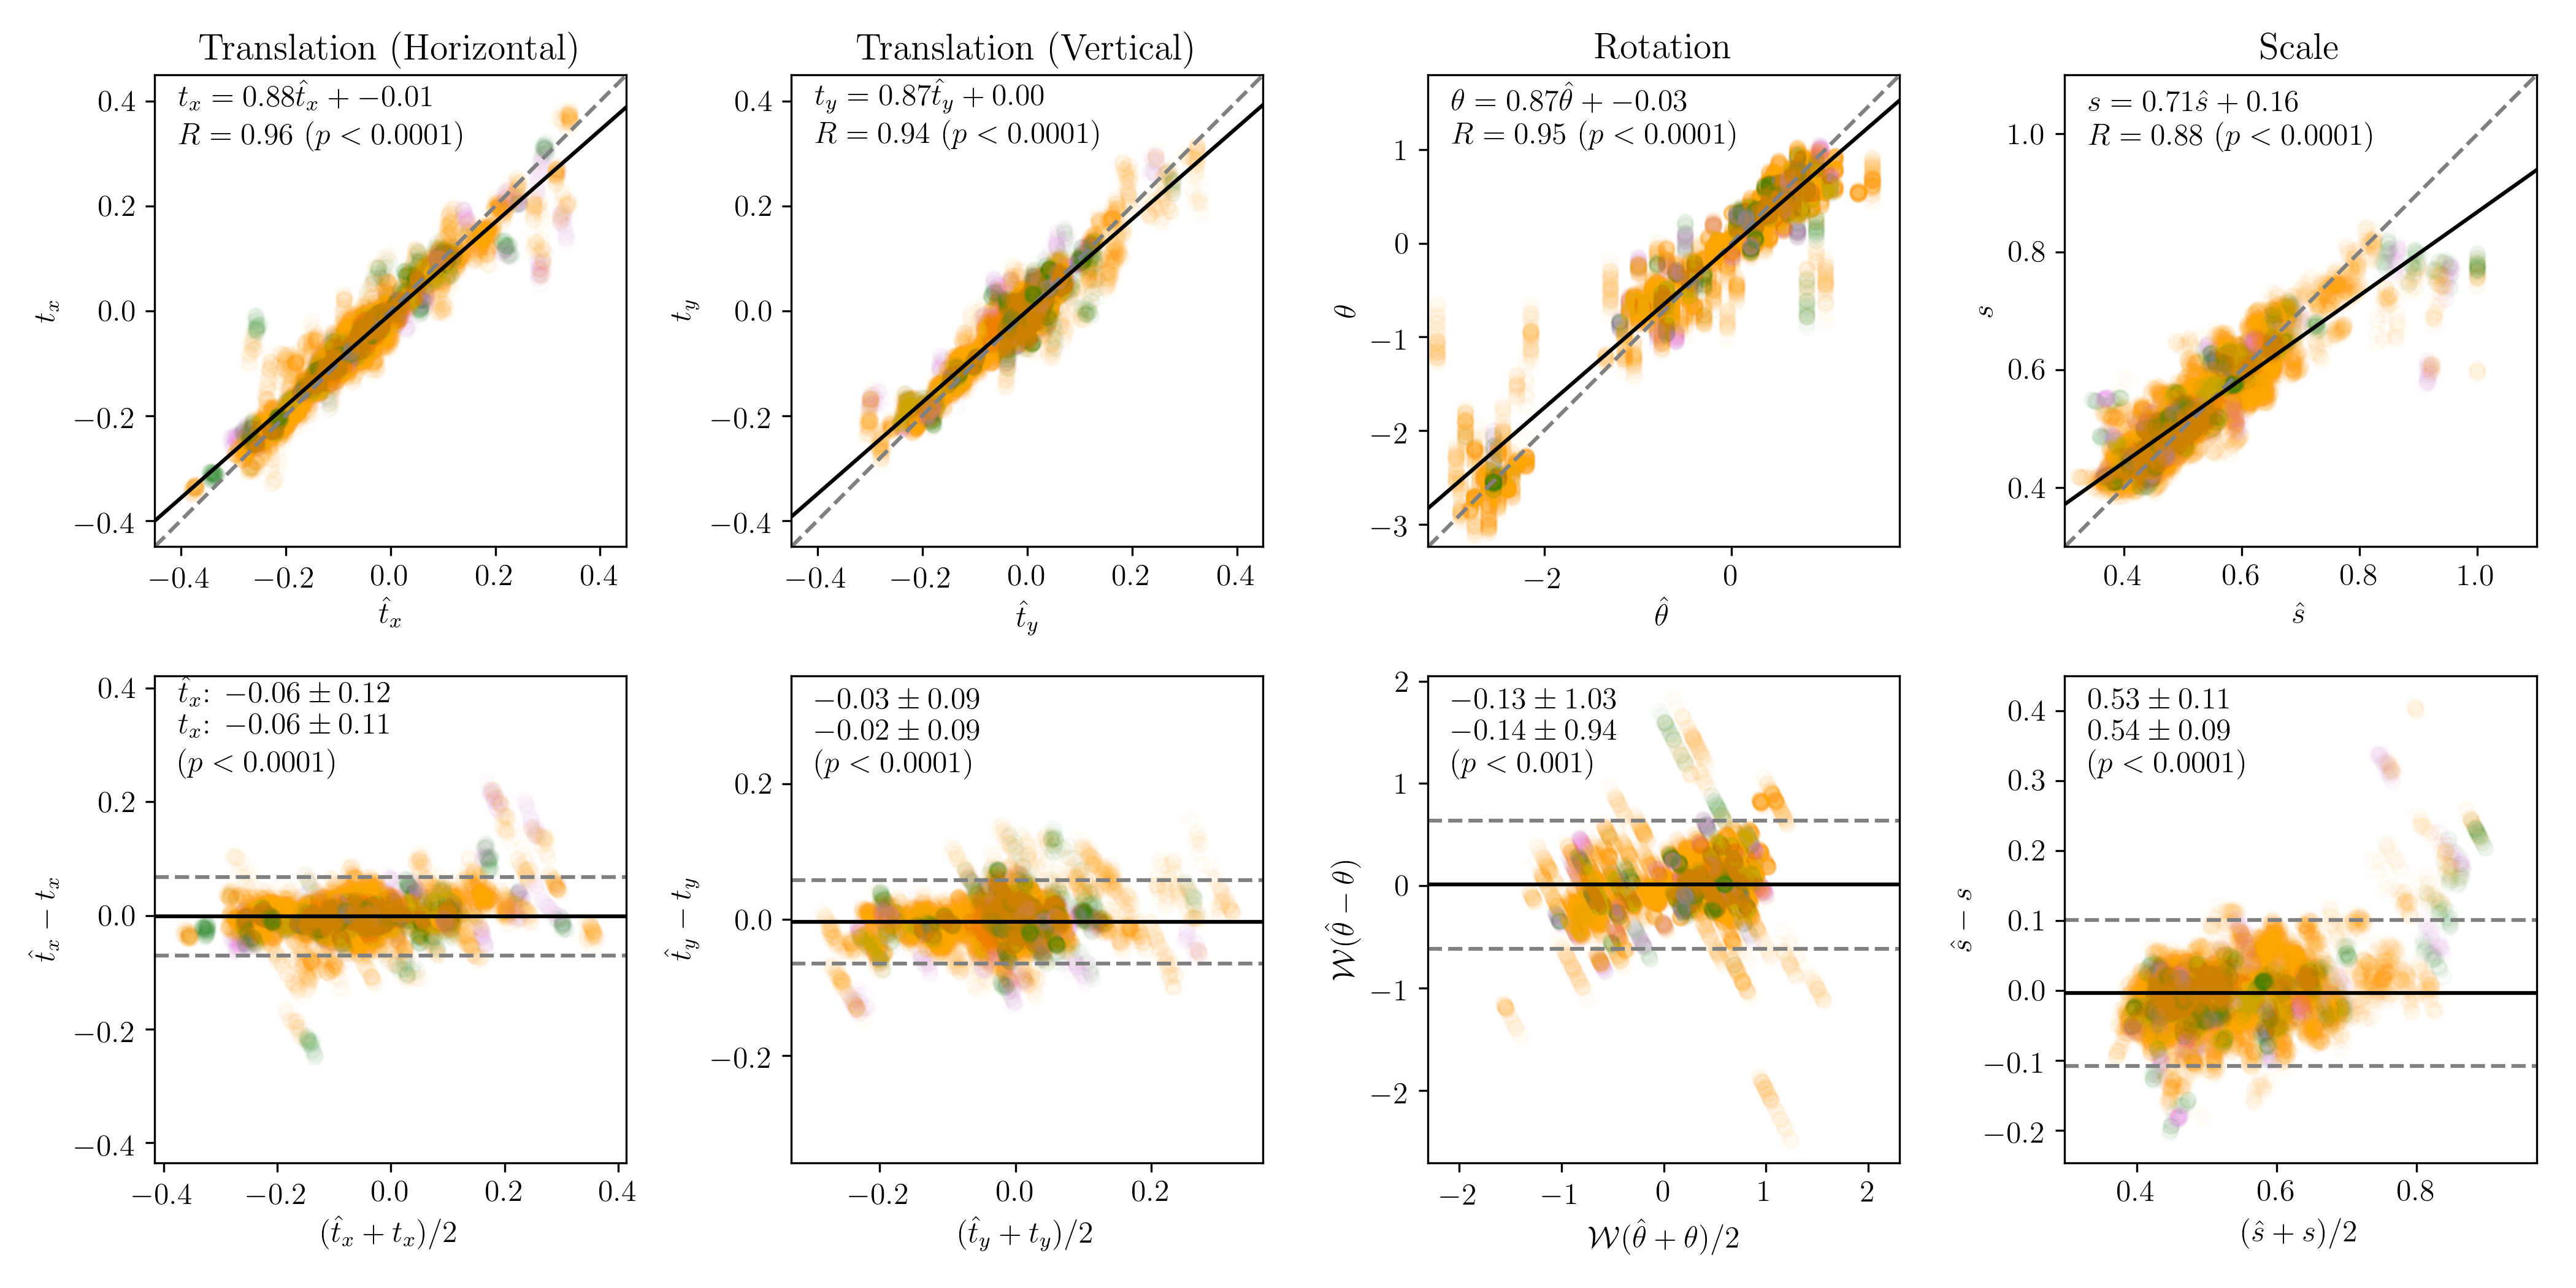
\includegraphics[width=1.0\textwidth]{./data/matrix-loss.png}
\caption[\captiontitle]{\captiontitle{}.
我们给出了变换参数的预测值与真实值之间的相关系数图(上)和 Bland-Altman 图(下).
\SA{}、\HLA{} 和 \VLA{} 误差分贝用橙色、绿色和紫色点表示(所有的点都做了半透明处理,以方便查看).
在相关系数图中,最佳的拟合线用黑色实线表示,理想的线条($y = x$)用灰色的虚线表示.
我们也给出了拟合线的公式和皮尔森相关系数 $R$.
而在 Bland-Altman 图中,误差均值用黑色水平实线表示,$\pm 1.96$ 的标准差界线用灰色水平虚线表示.
}
\label{fig:matrix-loss}
\end{center}
\end{sidewaysfigure*}

